\documentclass{beamer}
\usepackage{listings}
\usetheme{Copenhagen}
\usecolortheme{beaver}
\setbeamertemplate{navigation symbols}{}
\setbeamertemplate{footline}{\parbox[t][12pt][c]{12pt}{~\scriptsize\insertframenumber}}
% \usepackage{beamerthemesplit} // Activate for custom appearance

%%%%%%%%%%%%
% MVS: Language definitions
%
\renewcommand{\ttdefault}{pcr}
\lstset{
  basicstyle=\small\ttfamily,
  breaklines=true
}
\lstdefinelanguage{cvl}{
  morekeywords={generalize,to, with, other, at, zoom, levels, weigh, by, subject, and, create, constraint, as, not, exists, resolve, if, delete, select, from, where, in, order, over, setup, teardown,force,min,level,for,allornothing,join,on,setup,group,having,index,temporary,table,drop,partition,merge,partitions},
  sensitive=false,
  morecomment=[l]{//},
  morecomment=[s]{/*}{*/},
  morestring=[b]",
}
\lstset{
  language=cvl
}



\title{Declarative Cartography}
\subtitle{In-Database Map Generalization of Spatial Datasets}
\author{\underline{Pimin Konstantin Kefaloukos}, Marcos Vaz Salles, \\Martin Zachariasen\\ \small{\emph{Computer Science Department (DIKU)}, \textbf{University of Copenhagen}}}
\date{\today}

\begin{document}

\frame{\titlepage}

% MOTIVATION
\frame
{
  \frametitle{Overview}
  \begin{center}
  \fbox{A view of digital web maps today :-) }
  \end{center}
  
  \begin{itemize}
  \item \textbf{OK}: Background maps are stable and of good quality (commercial and national map providers)
  \item \textbf{Challenge}: New thematic data is constantly emerging and changing (social media, sensors, ...)
  \item \textbf{Goal}: Design \emph{easy-to-use}, \emph{cheap}, \emph{scalable} and \emph{effective} method for \underline{generalizing}, \underline{serving} and \underline{visualizing} thematic data
  \item \textbf{Use cases}: Data journalism, citizen information systems, crisis response, social media, ...
  \end{itemize}

}

\frame
{
  \frametitle{Map Generalization 101}
  Transforming raw spatial data\footnote{Tourism points-of-interest from OpenStreetMap}
  \begin{center}
  \fbox{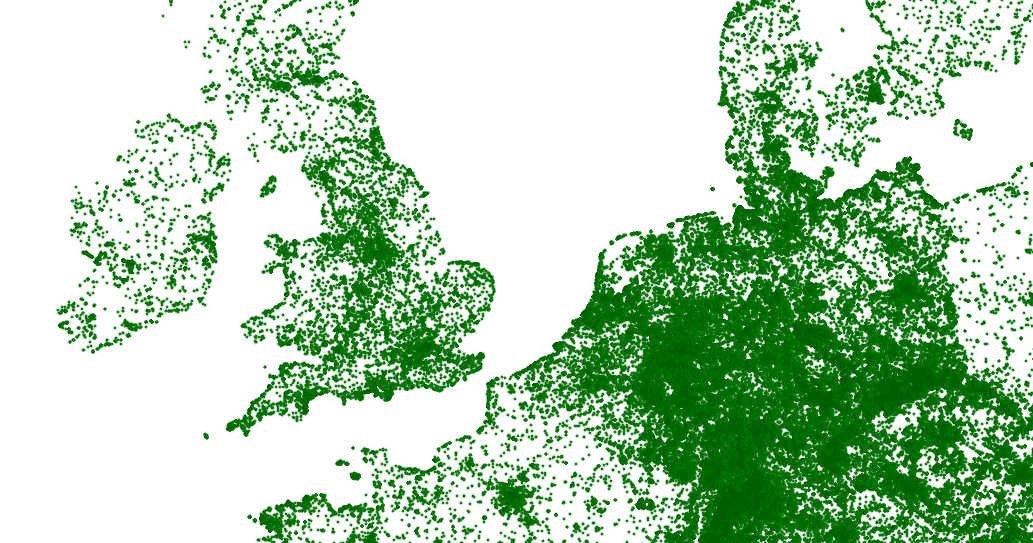
\includegraphics[scale=0.12]{figs/toomanyobjects.png}}
  \end{center}
  Into legible maps\footnote{Map created using simple random sampling of thematic point data}
  \begin{center}
  \fbox{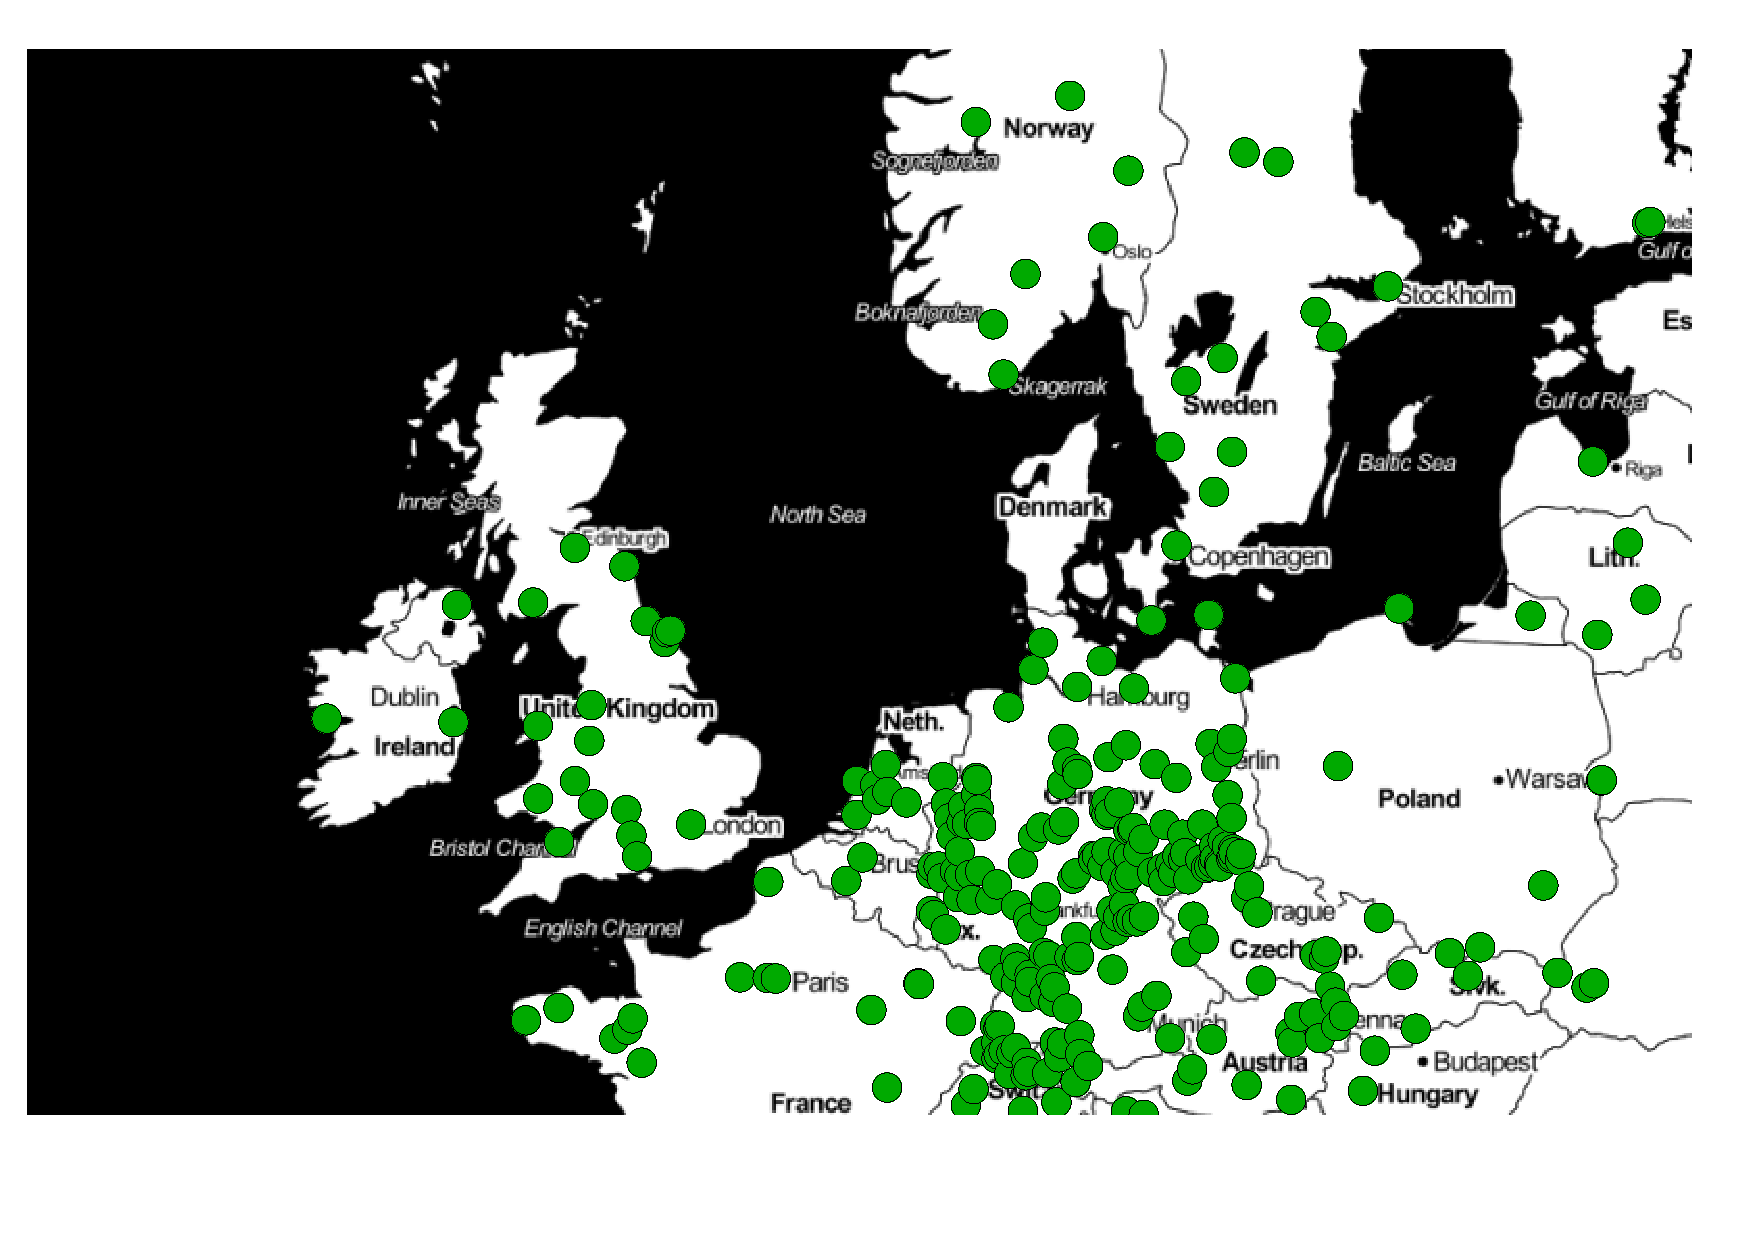
\includegraphics[scale=0.15]{figs/generalized-tourism.pdf}}
  \end{center}
}

\frame
{
  \frametitle{Questions pt 1}
  \begin{itemize}
  \item Decades of research in efficient algorithms for \emph{non}-spatial problems (Shortest Path, Travelling Salesman, Set Cover)
  \item Good algorithms exist for specific generalization problems\footnote{CS view, maybe geographers have knowledge to share here}~\cite{fusiontables,landcover}
  \item \textbf{Question}: Can we transform several related map generalization problems into a \emph{non}-spatial problem and reuse existing algorithms for this problem?
  \item \textbf{Question}: What is a good non-spatial problem to use?
  \end{itemize}
  
  \begin{center}
  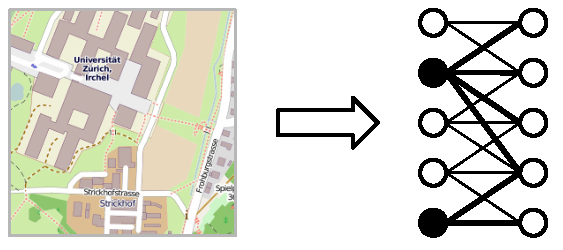
\includegraphics[scale=0.6]{figs/cvl-spatial-to-nonspatial.pdf}
  \end{center}
}

\frame
{
  \frametitle{Questions pt 2}
  \begin{itemize}
  \item A spatial database is a natural place to store spatial records
  \item However, map generalization algorithms are often implemented in specialized \emph{external software}, e.g. a Java program $\implies$ \emph{moving data in and out of database}
  \item Decades of research in database optimization
  \item Functionality includes \texttt{JOIN}, \texttt{ORDER BY}, \texttt{GROUP BY},  \texttt{CREATE INDEX} and many spatial functions: \texttt{ST\_Intersects}, \texttt{ST\_Distance}, ...
  \item \textbf{Question}: Can we formulate map generalization algorithms as a SQL transaction (with stored procedures) to be executed efficiently by a \emph{spatial database}?
  \end{itemize}
}

\begin{frame}[fragile]
  \frametitle{Questions pt 3}
  \begin{itemize}
  \item Writing complex queries in SQL is hard
  \item \textbf{Question}: Can we design a simple language that is compiled into complex SQL?
\begin{lstlisting}
GENERALIZE 
   restaurants TO restaurants2
AT 20 ZOOM LEVELS
WEIGH BY
  star_rating
SUBJECT TO 
   proximity 10
\end{lstlisting}
  \end{itemize}
\end{frame}


\frame
{
  \frametitle{Our approach}
  \begin{itemize}
  \item \textbf{Optimization}: Fit thematic generalization problem to well-known \emph{optimization problem}, i.e. \emph{set multicover problem}
  \item \textbf{Algorithms}: Survey \emph{existing algorithms} for this problem
  \item \textbf{Language}: Design an easy to use \emph{programming language} (CVL) for a class of generalization problems
  \item \textbf{Compile}: Compile CVL into a SQL transaction that generates and solves instances of the set multicover problem, and in turn solves the original generalization problem

  \end{itemize}
  \begin{center}
  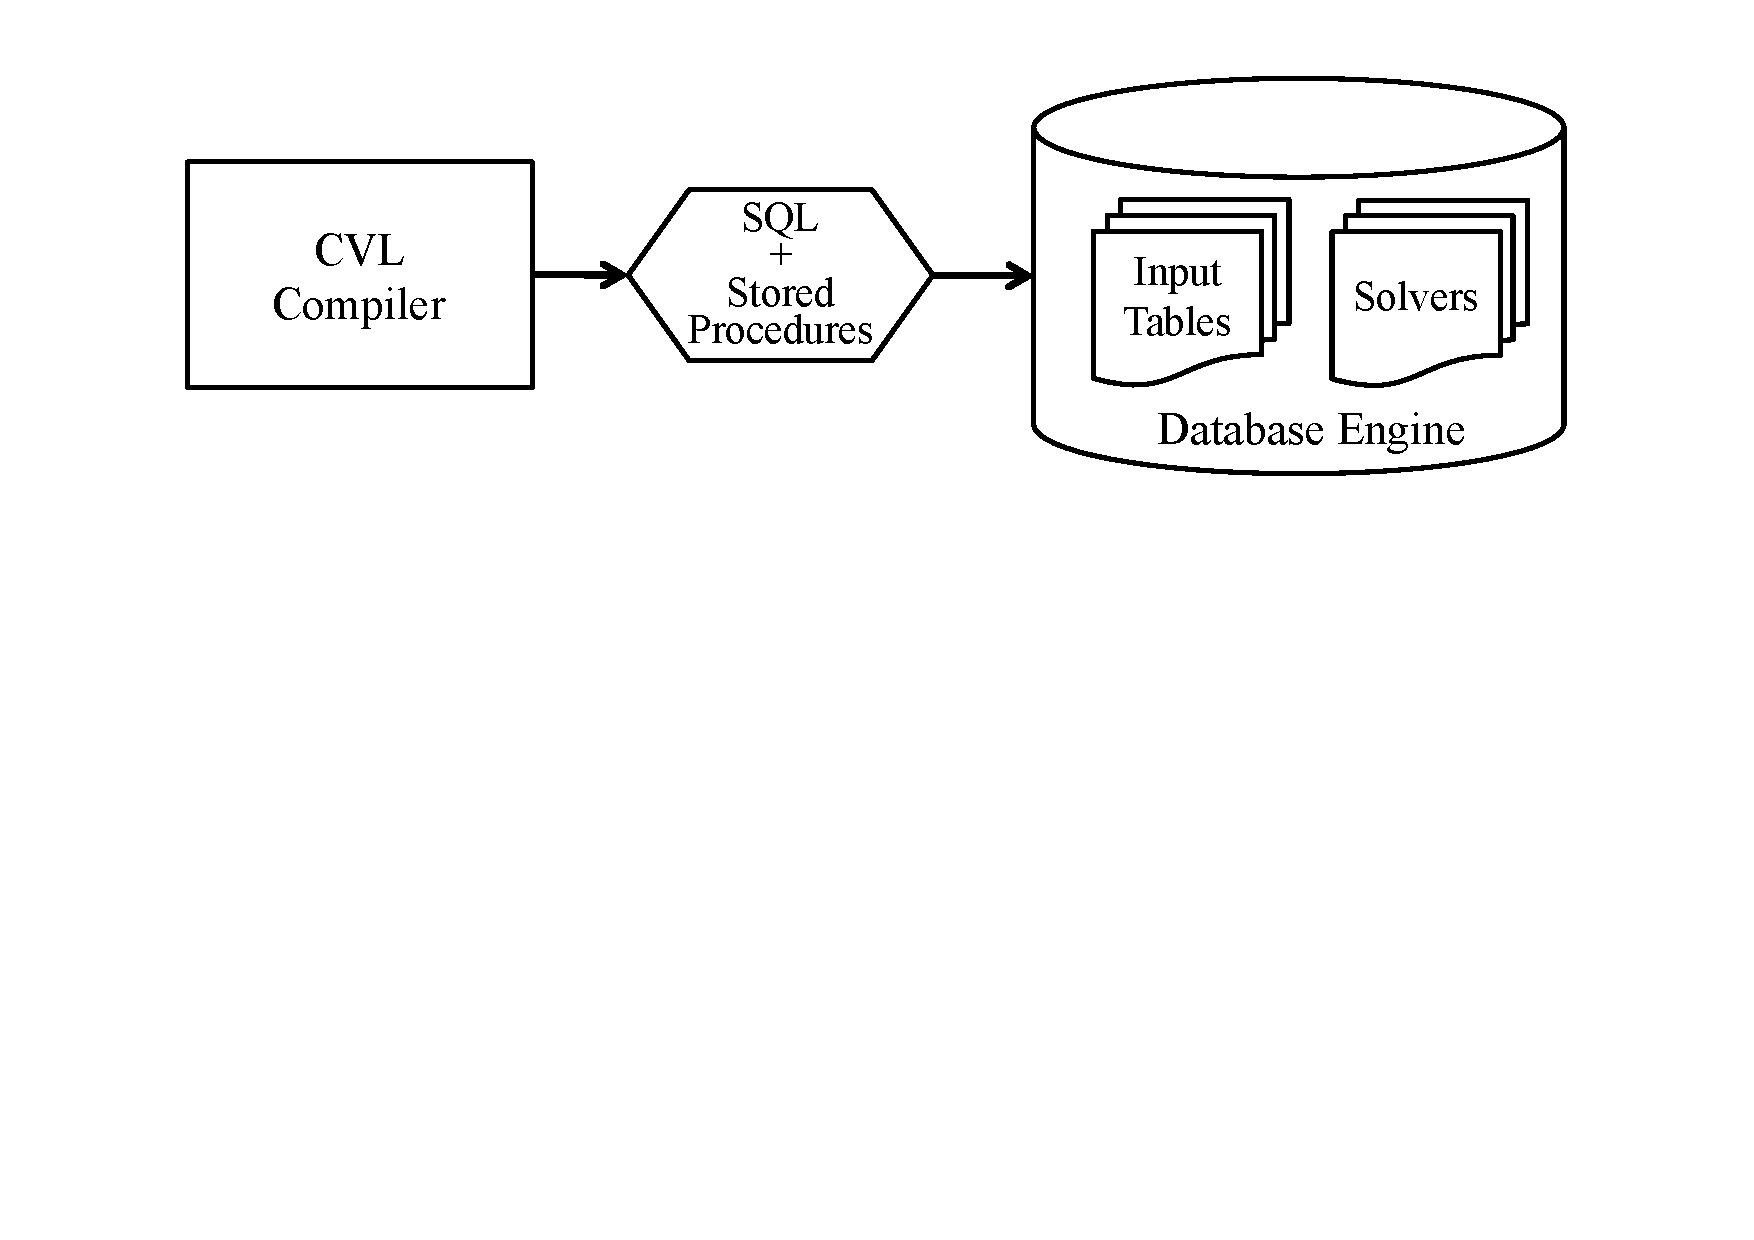
\includegraphics[scale=0.3]{figs/indatabase-execution.pdf}
  \end{center}
}


%\frame
%{
%  \frametitle{Relation to Reverse Data Management}

%  We implemented \emph{how-to} queries for spatial data:
%  \begin{itemize}
%  \item \textbf{How-to queries}~\cite{reversedatamanagement}: Given an \emph{input database}; compute an \emph{output database}, subject to set of \emph{constraints} and minimizing/maximizing an \emph{objective function}
%  \item \textbf{Spatial example}: Given an \emph{input database of spatial objects}; compute an output database that generalizes the objects to $\mathcal{Z}$ zoom-levels, subject to \emph{spatial constraints} and while \emph{minimizing loss} of objects in map (with prioritization)
%  \end{itemize}
%}

\frame
{
  \frametitle{Please note!}
  TODO: Eliminate this slide, it disrupts flow...
  
  Whenever you see the word \emph{``delete''} in this presentation, please append the words \emph{``or aggregate (future work)''} in your mind. \\
  making grammatical adjustments where appropriate.
  
  \begin{center}
  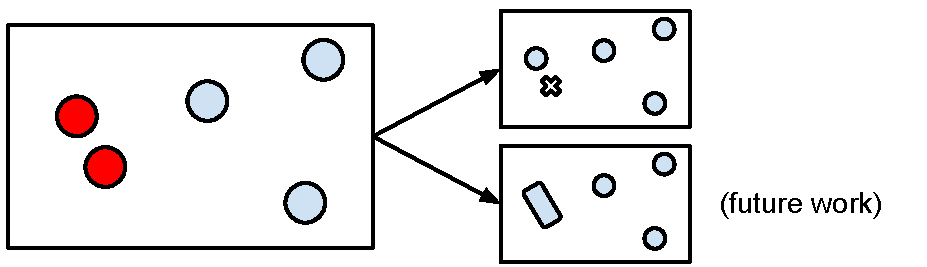
\includegraphics[scale=0.50]{figs/cvl-delete-aggregate.pdf}
  \end{center}
}


\frame
{
  \frametitle{Multi-scale filtering problem}
  \begin{itemize}
  \item Each record in database has a user-defined ``weight'' which models the importance of the record
  \item For each record we must pick a minimum zoom-level from which the records appears in the map
  \item We must minimize the aggregate weight over all zoom-levels of records that are filtered out
  \item At each zoom-level we must satisfy a set of constraints
  \end{itemize}
  \begin{center}
  \fbox{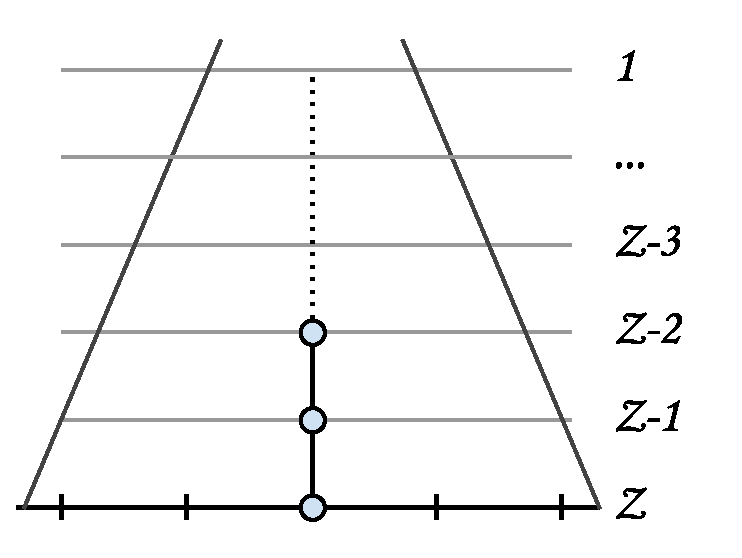
\includegraphics[scale=0.4]{figs/cvl-problem.pdf}}
  \end{center}
}


\frame
{
  \frametitle{Spatial constraints considered}
  \begin{itemize}
  \item \textbf{Zoom-consistency} (always enforced):  If an object is filtered out on a given zoom-level, it must also be filtered out on all lower zoom-levels
  \item \textbf{Proximity constraint} (user defined): Any pair of objects must be separated by minimum distance
  \item \textbf{Visibility constraint} (user defined): At most $K$ objects may be visible within a cell
  \end{itemize}
  \begin{center}
  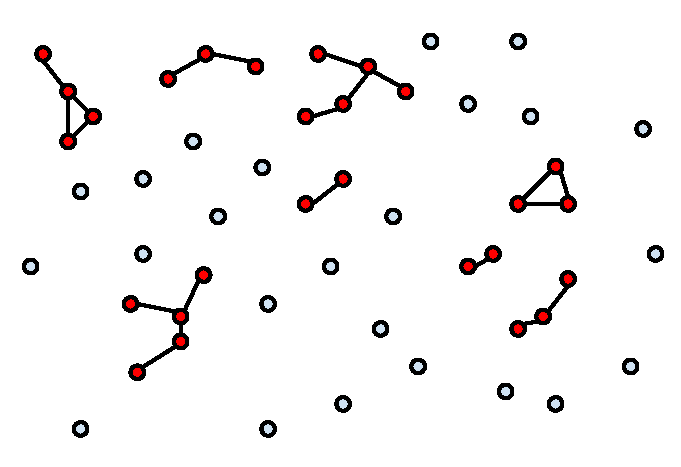
\includegraphics[scale=0.4]{figs/cvl-proximity.pdf} 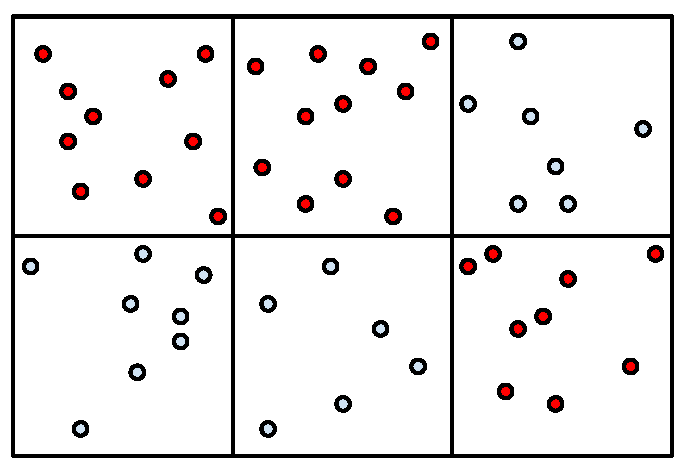
\includegraphics[scale=0.4]{figs/cvl-visibility.pdf}
  \end{center}
}


\frame
{
  \frametitle{Conflict sets}
  \begin{itemize}
  \item Model constraints (visibility, proximity, ...) using the notion of \emph{conflict sets}
  \item A conflict set is a \emph{set of objects} that cannot all appear simultaneously at a given zoom level
  \item An object can be in several conflict sets
  \item In a conflict set consisting of $k_1$ objects, where at most $k_2$ may appear in map, $\lambda = k_2 - k_1$ objects must be filtered out (deleted from current and lower zoom-levels)
  \end{itemize}
  \begin{center}
  	\fbox{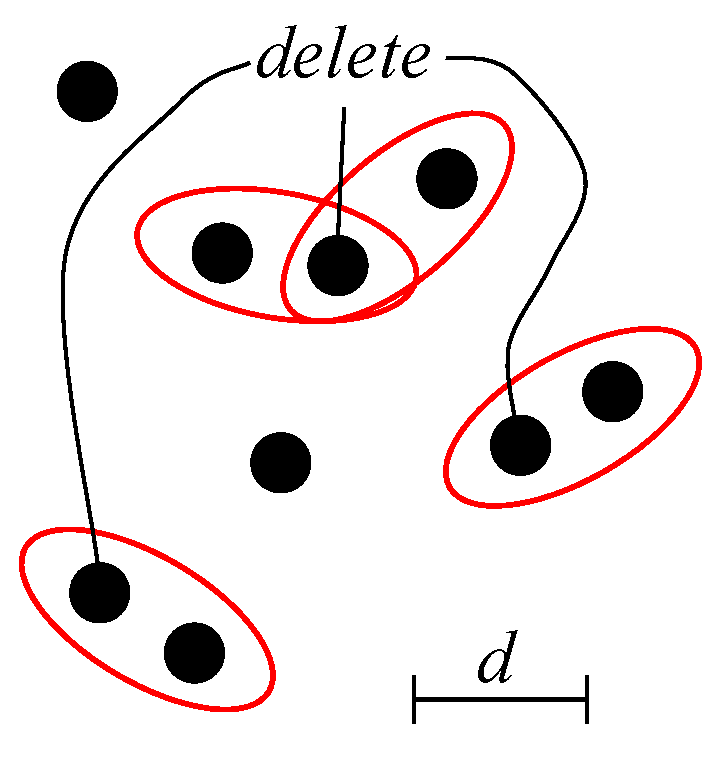
\includegraphics[scale=0.20]{figs/cvl-proximity-conflicts-2.pdf}} \fbox{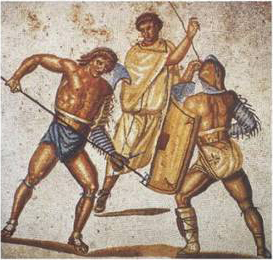
\includegraphics[scale=.38]{figs/gladiators.jpg}} \fbox{
\includegraphics[scale=.288]{figs/the-godfather-1.jpg}}
  \end{center}
}

\frame
{
  \frametitle{Single-scale filtering problem $\Leftrightarrow$ Set multicover problem}

  For each zoom-level we seek an optimal solution:

  \begin{itemize}
  \item \textbf{Set cover problem}: Given a universe $U$ of elements and a set $S$ of subsets of $U$, a \emph{cover} is a set $Q \subseteq S$ such that the union of $Q$ equals $U$.
  \item \textbf{Set multicover problem}: Each element in $e \in U$ has to be covered multiple times by $Q$.
  \item \textbf{Single-scale filtering problem}: Each conflict set $c \in C$ has to be covered multiple times times by objects that are filtered out.
  \end{itemize}
}


\begin{frame}[fragile]
\frametitle{Declarative Language for Generalization (CVL)}

\begin{itemize}
\item Language has two statements: \emph{Generalize} and \emph{Create Constraint}
\item A \emph{Generalize} statement can reference constraints defined in a \emph{Create Constraint} statement
\item Language is visually similar to SQL and uses snippets of embedded SQL
\item Designed to be compiled into SQL and executed in a database (where the data is assumed to be stored)
\end{itemize}
\end{frame}


\begin{frame}[fragile]
\frametitle{CVL: Generalize statement}
\begin{lstlisting}
GENERALIZE 
   restaurants TO restaurants_generalized
AT 20 ZOOM LEVELS
WEIGH BY
  star_rating
SUBJECT TO 
   proximity 10 AND
   visibility 64
\end{lstlisting}

\begin{itemize}
\item \texttt{restaurants} is an existing database table
\item \texttt{restaurants\_generalized} will be computed  
\item \texttt{star\_rating} used as object weight (any valid SQL expression)
\item \texttt{proximity} and \texttt{visibility} references constraints
\end{itemize}

\end{frame}

\begin{frame}[fragile]
\frametitle{CVL: Create Constraint}
\begin{lstlisting}
CREATE CONSTRAINT {Name, e.g. Proximity}
AS NOT EXISTS
  {SQL select statement}
  
RESOLVE cid IF DELETE (
  {integer expression}
)
\end{lstlisting}

\begin{itemize}
\item Select statement should return two result columns: \texttt{cid} (conflict ID) and \texttt{rid} (object ID)
\item Proximity constraint: the SQL select statement is a two-way spatial distance join that finds all objects that are too close
\item Proximity constraint: the integer expression is the constant $1$
\end{itemize}

\end{frame}

\begin{frame}[fragile]
\frametitle{Defining the proximity constraint (experts only)}
\begin{lstlisting}
CREATE CONSTRAINT Proximity
AS NOT EXISTS (
  SELECT l.{rid} || r.{rid} AS cid, Unnest(array[l.{rid}, r.{rid}]) AS rid
  FROM
    {level_view} l JOIN {level_view} r
  ON
    l.{rid} < r.{rid}
  AND
    l.{geom} && ST_Expand(r.{geom}, CVL_Resolution({z}, 256) * {parameter_1})
  AND
    ST_Distance(l.{geom}, r.{geom}) < CVL_Resolution({z}, 256) * {parameter_1}
)

RESOLVE cid IF DELETE (
  1
)
\end{lstlisting}
\end{frame}

\begin{frame}[fragile]
\frametitle{Proximity constraint: the important part}
\begin{itemize}
\item The core of the proximity constraint is a two-way spatial join:
\end{itemize}
\begin{lstlisting}
SELECT
   ...
FROM 
   ... left JOIN ... right
ON 
   ST_Distance(left.the_geometry, right.the_geometry) < {meters}
\end{lstlisting}
\end{frame}





\frame
{
  \frametitle{Future work}
  \begin{itemize}
  \item Relax zoom-consistency: \emph{min} and \emph{max} zoom-level for records)
  \item Extend work with \emph{aggregation} in language (semantics) and algorithm (implementation)
  \item Implement compilation of CVL to a distributed database dialect
  \end{itemize}
}

\frame
{
  \frametitle{Future work: Aggregation}
  \begin{center}
  \fbox{This is where we need your help :-)}
  \end{center}

  \begin{itemize}
  \item \textbf{User-level semantics}:
  \begin{itemize}
  \item How should user \emph{understand} aggregation, e.g. aggregation of non-geometric attributes?
  \item How should user \emph{parameterize} aggregation?
  \end{itemize}
  \item \textbf{Implementation}:
  \begin{itemize}
  \item Can we \emph{stretch} the existing model to include aggregation?
  \item Else, how does aggregation \emph{change} the problem/model?
  \item Do we need new \emph{algorithms}?
  \end{itemize}
  \end{itemize}

  \begin{center}
  \fbox{\textbf{Eiffel Tower + Louvre = ?}}
  \end{center}

}



% RELATED WORK
\frame
{
  \frametitle{Related work}

  \begin{itemize}
  \item \emph{Efficient Spatial Sampling of Large Geographical Tables}. Das Sarma, A., Lee, H., Gonzalez, H., Madhavan, J., \& Halevy, A. (2012).
  \item \emph{Reverse data management}, Meliou, A., Gatterbauer, W., \& Suciu, D. (2011).
  \item \emph{Generalization of land cover maps by mixed integer programming}. Haunert, J.-H., \& Wolff, A. (2006). 
  \item \emph{Constant information density in zoomable interfaces}. Woodruff, A., Landay, J., Stonebraker, M. (1998).
  \item And tons more of course...
  \end{itemize}
}

% Past and future work
\frame
{
  \frametitle{Past and future work}

  \begin{itemize}
  \item Past work: \emph{TileHeat}, predicting where people will look on a map tomorrow
  \item Latest work: \emph{Declarative Cartography}, the work described in these slides
  \item Future work: \emph{Real-time Declarative Cartography}, joint work with people at University of Zurich (Department of Geography)
  \item Future work: Succinct data representation of high-fidelity spatial data that is visualized on a digital map on a screen (think: pixel precision is not all that good)
  \end{itemize}
}




\end{document}
